\section{Деление многочленов, интерполяция и линейные рекурренты}

На прошлой лекции мы научились перемножать два многочлена степени $n$ за время $O(n \log n)$ с помощью Быстрого преобразования Фурье. Сегодня мы увидим, что быстрое умножение многочленов служит ключом к целому семейству алгебраических операций: обращению степенных рядов, делению многочленов с остатком, вычислению многочлена сразу в $m$ произвольных точках, интерполяции и быстрому вычислению $n$-го члена линейных рекуррентных последовательностей.

На протяжении всей лекции будем считать, что коэффициенты многочленов лежат в конечном поле $\Z_p$ (где $p = b \cdot 2^a + 1$ "--- простое число, допускающее теоретико-числовое преобразование Фурье).

\subsection{Обратный ряд по модулю \texorpdfstring{$x^m$}{x\^m} за \texorpdfstring{$O(m \log m)$}{O(m log m)}}

В кольце многочленов $\Z_p[x]$ обратимы только ненулевые константы: у многочлена положительной степени не бывает обратного многочлена. Однако если мы работаем \textbf{по модулю $x^m$} (то есть в факторкольце $\Z_p[x] / (x^m)$, отбрасывая все мономы степени $m$ и выше), то обратимыми становятся почти все многочлены.

\begin{definition}
    Пусть дан многочлен (или формальный степенной ряд) $P(x) = a_0 + a_1 x + a_2 x^2 + \dots$ Многочлен $Q(x)$ степени $< m$ называется \textbf{обратным к $P(x)$ по модулю $x^m$} и обозначается $P(x)^{-1} \bmod x^m$, если
    \[
        P(x) \cdot Q(x) \equiv 1 \pmod{x^m},
    \]
    то есть в произведении $P(x) Q(x)$ свободный член равен $1$, а коэффициенты при $x^1$, $x^2$, $\dots$, $x^{m-1}$ равны $0$.
\end{definition}

\begin{proposition}[Критерий обратимости по модулю $x^m$]
    Многочлен $P(x) = a_0 + a_1 x + \dots$ обратим по модулю $x^m$ тогда и только тогда, когда его свободный член отличен от нуля: $a_0 \ne 0$. При этом обратный многочлен степени $< m$ единственен.
\end{proposition}

\begin{proof}
    Если $P(x) Q(x) \equiv 1 \pmod{x^m}$, то при подстановке $x = 0$ получаем $a_0 \cdot Q(0) = 1$ в поле $\Z_p$, откуда $a_0 \ne 0$ и $Q(0) = a_0^{-1}$. Обратно, если $a_0 \ne 0$, мы сейчас предъявим явный алгоритм построения $Q(x)$ методом удвоения точности.
\end{proof}

Научимся находить $Q(x) = P(x)^{-1} \bmod x^m$ за время $O(m \log m)$. Достаточно уметь делать это для случая, когда $m = 2^k$ является степенью двойки (если $m$ не степень двойки, дополним его до ближайшей сверху степени двойки, а в конце отбросим лишние старшие коэффициенты).

\textbf{База ($m = 1$).} По модулю $x^1$ от многочлена $P(x)$ остаётся только свободный член $a_0 \ne 0$. Обратным к нему служит константа $Q_0(x) = a_0^{-1} \equiv a_0^{p - 2} \pmod p$, которую мы находим за $O(\log p)$ бинарным возведением в степень по малой теореме Ферма.

\textbf{Шаг удвоения точности ($m \to 2m$).} Пусть мы уже нашли многочлен $Q_0(x)$ степени $< m$, обратный к $P(x)$ по модулю $x^m$:
\[
    P(x) \cdot Q_0(x) \equiv 1 \pmod{x^m}.
\]
Как за $O(m \log m)$ получить из него многочлен $Q(x)$ степени $< 2m$, обратный к $P(x)$ по модулю $x^{2m}$?

Запишем первые $2m$ коэффициентов многочлена $P(x)$ в виде
\[
    P(x) \equiv P_0(x) + x^m P_1(x) \pmod{x^{2m}}, \qquad \text{где } \deg P_0, \deg P_1 < m.
\]
Так как $P_0(x) \equiv P(x) \pmod{x^m}$, произведение $P_0(x) Q_0(x)$ даёт остаток $1$ по модулю $x^m$, а его степень строго меньше $2m$. Значит, его можно записать в виде
\[
    P_0(x) Q_0(x) = 1 + x^m R(x),
\]
где $R(x)$ "--- известный нам многочлен степени $< m$ (достаточно перемножить $P_0$ и $Q_0$ с помощью БПФ и взять коэффициенты при степенях от $x^m$ до $x^{2m-1}$).

Искомый обратный многочлен $Q(x)$ по модулю $x^{2m}$ совпадает с $Q_0(x)$ в младших $m$ коэффициентах, поэтому будем искать его в виде
\[
    Q(x) = Q_0(x) + x^m Q_1(x), \qquad \deg Q_1 < m.
\]
Перемножим $P(x)$ и $Q(x)$ по модулю $x^{2m}$, замечая, что слагаемое $x^{2m} P_1(x) Q_1(x)$ делится на $x^{2m}$ и потому исчезает:
\begin{align*}
    P(x) Q(x) &\equiv \bigl(P_0(x) + x^m P_1(x)\bigr) \bigl(Q_0(x) + x^m Q_1(x)\bigr) \equiv \\
    &\equiv P_0(x) Q_0(x) + x^m \bigl(P_0(x) Q_1(x) + P_1(x) Q_0(x)\bigr) = \\
    &= 1 + x^m \bigl(R(x) + P_0(x) Q_1(x) + P_1(x) Q_0(x)\bigr) \pmod{x^{2m}}.
\end{align*}
Нам нужно, чтобы правая часть была сравнима с $1$ по модулю $x^{2m}$. Это равносильно тому, что выражение в скобках при $x^m$ делится на $x^m$:
\begin{gather*}
    R(x) + P_0(x) Q_1(x) + P_1(x) Q_0(x) \equiv 0 \pmod{x^m} \quad \Lra \\
    \Lra \quad P_0(x) Q_1(x) \equiv -\bigl(R(x) + P_1(x) Q_0(x)\bigr) \pmod{x^m}.
\end{gather*}
Но по модулю $x^m$ обратным к многочлену $P_0(x)$ является уже известный нам многочлен $Q_0(x)$. Домножая обе части сравнения на $Q_0(x)$ по модулю $x^m$, выражаем неизвестную старшую половину $Q_1(x)$:
\begin{equation}\label{eq:poly_inv_step}
    Q_1(x) \equiv -Q_0(x) \cdot \bigl(R(x) + P_1(x) Q_0(x)\bigr) \pmod{x^m}.
\end{equation}
\begin{note}
    Если подставить $x^m R(x) = P_0(x) Q_0(x) - 1$ обратно в формулу для $Q(x) = Q_0(x) + x^m Q_1(x)$, мы получим классическую формулу \textbf{метода Ньютона} для уравнения $f(Q) = Q^{-1} - P = 0$:
    \[
        Q(x) \equiv Q_0(x) \cdot \bigl(2 - P(x) Q_0(x)\bigr) \pmod{x^{2m}}.
    \]
\end{note}

\begin{theorem}
    Вычисление обратного ряда $P(x)^{-1} \bmod x^m$ методом удвоения работает за время $O(m \log m)$.
\end{theorem}

\begin{proof}
    Переход от $m$ к $2m$ по формуле~\eqref{eq:poly_inv_step} требует константного числа перемножений многочленов степени $< m$ с помощью БПФ, то есть работает за $O(m \log m)$. Суммируя время работы по всем уровням удвоения $1, 2, 4, \dots, m = 2^k$, получаем геометрическую прогрессию:
    \[
        \sum_{j=0}^k O(2^j \cdot j) \le O(k) \cdot \sum_{j=0}^k 2^j = O(k \cdot 2^{k+1}) = O(m \log m).
    \]
\end{proof}

\subsection{Деление многочленов с остатком за \texorpdfstring{$O(n \log n)$}{O(n log n)}}

Научившись обращать многочлены по модулю $x^m$, мы можем за $O(n \log n)$ выполнять обычное \textbf{деление многочленов уголком с остатком}.

Пусть даны делимое $F(x)$ степени $n$ и делитель $G(x)$ степени $m \le n$ (со старшим коэффициентом $g_m \ne 0$). Требуется найти частное $Q(x)$ ($\deg Q = n - m$) и остаток $R(x)$ ($\deg R < m$), удовлетворяющие тождеству
\begin{equation}\label{eq:poly_div}
    F(x) = G(x) \cdot Q(x) + R(x).
\end{equation}

Введём операцию \textbf{разворота коэффициентов} многочлена. Для любого многочлена $P(x) = p_0 + p_1 x + \dots + p_d x^d$ степени $d$ положим
\[
    \rev(P)(x) = x^d P\!\left(\frac{1}{x}\right) = p_d + p_{d-1} x + \dots + p_1 x^{d-1} + p_0 x^d.
\]
Подставим в равенство~\eqref{eq:poly_div} вместо $x$ дробь $\frac{1}{x}$ и умножим обе части на $x^n$. Поскольку $n = \deg F = \deg G + \deg Q$, получаем:
\[
    x^n F\!\left(\frac{1}{x}\right) = \left(x^{\deg G} G\!\left(\frac{1}{x}\right)\right) \cdot \left(x^{\deg Q} Q\!\left(\frac{1}{x}\right)\right) + x^{n - \deg R} \cdot \left(x^{\deg R} R\!\left(\frac{1}{x}\right)\right),
\]
что переписывается через развёрнутые многочлены как
\begin{equation}\label{eq:poly_div_rev}
    \rev(F)(x) = \rev(G)(x) \cdot \rev(Q)(x) + x^{n - \deg R} \rev(R)(x).
\end{equation}

Обратим внимание на множитель $x^{n - \deg R}$ перед остатком. Так как степень остатка строго меньше степени делителя ($\deg R < m \implies \deg R \le m - 1$), показатель степени $n - \deg R$ удовлетворяет оценке
\[
    n - \deg R \ge n - m + 1.
\]
Значит, если мы рассмотрим равенство~\eqref{eq:poly_div_rev} \textbf{по модулю $x^{n - m + 1}$}, слагаемое с остатком $x^{n - \deg R} \rev(R)(x)$ полностью занулится, и мы получим сравнение без остатка:
\[
    \rev(F)(x) \equiv \rev(G)(x) \cdot \rev(Q)(x) \pmod{x^{n - m + 1}}.
\]
При этом свободный член развёрнутого делителя $\rev(G)(x)$ равен старшему коэффициенту исходного делителя $g_m \ne 0$. Поэтому многочлен $\rev(G)(x)$ обратим по модулю $x^{n - m + 1}$, и мы можем выразить $\rev(Q)(x)$:
\[
    \rev(Q)(x) \equiv \rev(F)(x) \cdot \bigl(\rev(G)(x)\bigr)^{-1} \pmod{x^{n - m + 1}}.
\]
Но степень частного $Q(x)$ равна $n - m$, а значит, степень многочлена $\rev(Q)(x)$ также не превосходит $n - m$. Поэтому его остаток по модулю $x^{n - m + 1}$ совпадает с самим многочленом $\rev(Q)(x)$ без всякой потери старших коэффициентов.

Таким образом, алгоритм деления $F(x)$ на $G(x)$ с остатком состоит из четырёх шагов:
\begin{enumerate}
    \item Развернуть коэффициенты $F$ и $G$, получив $\rev(F)$ и $\rev(G)$.
    \item Найти обратный ряд $H(x) = (\rev(G)(x))^{-1} \bmod x^{n - m + 1}$ за время $O((n - m) \log(n - m))$.
    \item Перемножить $\rev(F)(x)$ и $H(x)$ по модулю $x^{n - m + 1}$ с помощью БПФ и развернуть первые $n - m + 1$ коэффициентов обратно, получив точное частное $Q(x)$.
    \item Вычислить остаток по формуле $R(x) = F(x) - G(x) \cdot Q(x)$ с помощью одного умножения БПФ за $O(n \log n)$.
\end{enumerate}

\subsection{Вычисление многочлена в \texorpdfstring{$m$}{m} точках за \texorpdfstring{$O(m \log^2 m)$}{O(m log\^2 m)}}

С помощью быстрого деления с остатком можно вычислить значения многочлена $P(x)$ степени $< m$ в $m$ \emph{произвольных} точках $x_1, x_2, \dots, x_m \in \Z_p$ за время $O(m \log^2 m)$.

По теореме Безу остаток от деления многочлена $P(x)$ на линейный двучлен $(x - x_i)$ равен константе $P(x_i)$:
\[
    P(x_i) = P(x) \bmod (x - x_i).
\]
Если делить $P(x)$ на каждый двучлен $(x - x_i)$ по отдельности, мы потратим $O(m)$ на каждую точку и $O(m^2)$ суммарно. Чтобы объединить вычисления, воспользуемся простым свойством остатков: если многочлен $M(x)$ делится нацело на многочлен $D(x)$, то
\[
    P(x) \bmod D(x) = \bigl(P(x) \bmod M(x)\bigr) \bmod D(x).
\]

Построим над набором точек $x_1, \dots, x_m$ бинарное \textbf{дерево отрезков из многочленов}:
\begin{enumerate}
    \item \textbf{Фаза 1 (построение снизу вверх):} в $i$-й лист дерева запишем многочлен первой степени $M_{i, i}(x) = x - x_i$. В каждую внутреннюю вершину, отвечающую отрезку $[l, r]$ со средним индексом $\text{mid} = \lfloor (l + r) / 2 \rfloor$, запишем произведение многочленов её левого и правого сыновей:
    \[
        M_{l, r}(x) = M_{l, \text{mid}}(x) \cdot M_{\text{mid}+1, r}(x) = \prod_{i=l}^r (x - x_i),
    \]
    вычисляя это произведение с помощью БПФ. На одном уровне дерева суммарная степень всех многочленов равна $m$, поэтому перемножения на одном уровне занимают $O(m \log m)$ времени, а построение всех $\lceil \log_2 m \rceil$ уровней дерева работает за $O(m \log^2 m)$.

    \begin{center}
    \begin{tikzpicture}[
        level distance=1.15cm,
        level 1/.style={sibling distance=5.6cm},
        level 2/.style={sibling distance=2.8cm},
        every node/.style={rectangle, rounded corners=3pt, draw=black!80, thick, fill=NavyBlue!10, inner sep=4pt, font=\footnotesize},
        edge from parent/.style={draw=black!80, -Stealth, thick}
    ]
        \node {$(x - x_1)(x - x_2)(x - x_3)(x - x_4)$}
            child { node {$(x - x_1)(x - x_2)$}
                child { node {$(x - x_1)$} }
                child { node {$(x - x_2)$} }
            }
            child { node {$(x - x_3)(x - x_4)$}
                child { node {$(x - x_3)$} }
                child { node {$(x - x_4)$} }
            };
    \end{tikzpicture}
    \par\nopagebreak\medskip
    \small\textit{Рис. 8.1. Дерево произведений линейных двучленов при $m = 4$.}
    \end{center}

    \item \textbf{Фаза 2 (спуск остатков сверху вниз):} для каждой вершины $[l, r]$ дерева вычислим многочлен-остаток
    \[
        P_{l, r}(x) = P(x) \bmod M_{l, r}(x), \qquad \deg P_{l, r} < r - l + 1.
    \]
    В корне дерева остаток $P_{1, m}(x) = P(x) \bmod M_{1, m}(x)$ равен самому $P(x)$ (так как $\deg P < m$). Далее, зная остаток $P_{l, r}(x)$ в вершине $[l, r]$, мы находим остатки в её сыновьях двумя быстрыми делениями многочленов с остатком:
    \[
        P_{l, \text{mid}}(x) = P_{l, r}(x) \bmod M_{l, \text{mid}}(x), \qquad P_{\text{mid}+1, r}(x) = P_{l, r}(x) \bmod M_{\text{mid}+1, r}(x).
    \]
    Поскольку при этом мы делим многочлен степени $< r - l + 1$ на многочлен половинной степени, работа в вершине $[l, r]$ составляет $O((r - l) \log(r - l))$. Когда спуск доходит до листа $[i, i]$, многочлен $P_{i, i}(x) = P(x) \bmod (x - x_i)$ имеет степень $0$ "--- это и есть искомое число $P(x_i)$.
\end{enumerate}
На каждом из $\lceil \log_2 m \rceil$ уровней дерева суммарное время делений составляет $O(m \log m)$, откуда общее время работы алгоритма равно $O(m \log^2 m)$.

\subsection{Интерполяция многочлена за \texorpdfstring{$O(n \log^3 n)$}{O(n log\^3 n)}}

Решим теперь обратную задачу: пусть заданы $n$ точек $(x_1, y_1), (x_2, y_2), \dots, (x_n, y_n)$, где все абсциссы $x_i$ попарно различны. Требуется найти коэффициенты единственного многочлена $P(x)$ степени $< n$, принимающего в этих точках заданные значения: $P(x_i) = y_i$ ($i = 1, \dots, n$).

Классическая интерполяционная формула Лагранжа
\[
    P(x) = \sum_{i=1}^n y_i \prod_{j \ne i} \frac{x - x_j}{x_i - x_j}
\]
при наивном вычислении требует $O(n^2)$ операций. Покажем, как построить $P(x)$ методом <<разделяй и властвуй>> за $O(n \log^3 n)$ (считая $n$ степенью двойки):

\begin{enumerate}
    \item Разделим множество из $n$ точек пополам и рекурсивно построим многочлен $P_1(x)$ степени $< n / 2$, который интерполирует первую половину точек:
    \[
        P_1(x_i) = y_i \qquad \text{для всех } i = 1, 2, \dots, \frac{n}{2}.
    \]
    \item Будем искать итоговый многочлен $P(x)$ степени $< n$ в виде
    \[
        P(x) = P_1(x) + R(x) \cdot Q(x), \qquad \text{где } R(x) = \prod_{i=1}^{n/2} (x - x_i).
    \]
    Заметим, что многочлен $R(x)$ обращается в нуль во всех точках первой половины ($R(x_i) = 0$ при $1 \le i \le n/2$). Поэтому при \emph{любом} выборе многочлена $Q(x)$ в первой половине точек равенство $P(x_i) = P_1(x_i) + 0 = y_i$ уже выполнено автоматически.

    \item Остаётся подобрать многочлен $Q(x)$ степени $< n / 2$ так, чтобы равенство $P(x_j) = y_j$ выполнилось и во второй половине точек ($j = n/2 + 1, \dots, n$). Подставляя $x = x_j$, получаем условие:
    \[
        P_1(x_j) + R(x_j) \cdot Q(x_j) = y_j \quad \Lra \quad Q(x_j) = \frac{y_j - P_1(x_j)}{R(x_j)} \qquad \left(j = \frac{n}{2} + 1, \dots, n\right).
    \]
    Поскольку все абсциссы $x_1, \dots, x_n$ попарно различны, знаменатель $R(x_j) = \prod_{i=1}^{n/2} (x_j - x_i)$ отличен от нуля при всех $j > n / 2$.

    \item Построим многочлен $R(x)$ и с помощью алгоритма многоточечного вычисления из предыдущего раздела за $O(n \log^2 n)$ найдём значения $P_1(x_j)$ и $R(x_j)$ во всех точках второй половины $x_{n/2+1}, \dots, x_n$. Вычислив целевые значения $z_j = (y_j - P_1(x_j)) \cdot R(x_j)^{-1}$, вторым рекурсивным вызовом найдём интерполяционный многочлен $Q(x)$ для точек $(x_j, z_j)$ ($j = n/2 + 1, \dots, n$), после чего вернём $P(x) = P_1(x) + R(x) Q(x)$.
\end{enumerate}

Время работы алгоритма удовлетворяет рекуррентному соотношению
\[
    T(n) = 2 T\!\left(\frac{n}{2}\right) + O(n \log^2 n),
\]
откуда $T(n) = O(n \log^3 n)$ (заметим также, что если построить дерево произведений $(x - x_i)$ один раз для всех $n$ точек заранее и использовать производную $M'(x_i)$ в формуле Лагранжа, время интерполяции можно сократить до $O(n \log^2 n)$).

\subsection{Линейные рекурренты за \texorpdfstring{$O(s \log s \log n)$}{O(s log s log n)}}

В заключение разберём одно из самых красивых применений полиномиальной арифметики "--- быстрое вычисление далёких членов линейных рекуррентных последовательностей.

Пусть заданы первые $s$ членов последовательности $a_0, a_1, \dots, a_{s-1}$ и фиксированные коэффициенты $c_0, c_1, \dots, c_{s-1}$, определяющие все последующие члены при $n \ge s$ по линейному рекуррентному соотношению порядка $s$:
\begin{equation}\label{eq:lin_rec}
    a_n = c_0 a_{n-s} + c_1 a_{n-s+1} + \dots + c_{s-1} a_{n-1}.
\end{equation}
Требуется вычислить $a_n \pmod p$ при большом $n$ (например, $n \sim 10^{18}$) и большом порядке рекурренты $s$ (например, $s \sim 10^5$).

\begin{example}
    Линейные рекурренты возникают в самых разных задачах:
    \begin{enumerate}
        \item \textbf{Числа Фибоначчи:} $F_n = F_{n-1} + F_{n-2}$ ($s = 2$, $c_0 = c_1 = 1$).
        \item \textbf{Треугольные числа} $a_n = \binom{n}{2}$ (и вообще любой многочлен степени $d$ от $n$): так как третьи конечные разности квадратичной функции равны нулю ($\Delta^3 a_n = a_n - 3a_{n-1} + 3a_{n-2} - a_{n-3} = 0$), последовательность удовлетворяет рекурренте $a_n = 3a_{n-1} - 3a_{n-2} + a_{n-3}$ порядка $s = 3$.
        \item \textbf{Числа Якобшталя и паросочетания в цепочке графов $K_4$:} рассмотрим граф, составленный из $n$ полных четырёхугольников $K_4$ (квадратов с обеими диагоналями), склеенных друг с другом по вертикальным боковым рёбрам в длинную полосу. Сколько в таком графе совершенных паросочетаний $a_n$?

        \begin{center}
        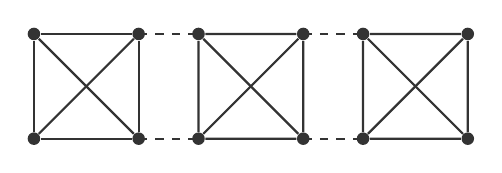
\begin{tikzpicture}[
            scale=0.95,
            v/.style={circle, fill=black!80, inner sep=1.6pt},
            e/.style={thick, black!80}
        ]
            \foreach \k in {0, 1, 2} {
                \pgfmathsetmacro{\x}{\k * 2.2}
                \node[v] (tl\k) at (\x, 1.4) {};
                \node[v] (bl\k) at (\x, 0) {};
                \node[v] (tr\k) at (\x + 1.4, 1.4) {};
                \node[v] (br\k) at (\x + 1.4, 0) {};
                \draw[e] (tl\k) -- (tr\k) -- (br\k) -- (bl\k) -- (tl\k);
                \draw[e] (tl\k) -- (br\k);
                \draw[e] (bl\k) -- (tr\k);
            }
            \draw[e, dashed] (1.4, 1.4) -- (2.2, 1.4);
            \draw[e, dashed] (1.4, 0) -- (2.2, 0);
            \draw[e, dashed] (3.6, 1.4) -- (4.4, 1.4);
            \draw[e, dashed] (3.6, 0) -- (4.4, 0);
        \end{tikzpicture}
        \end{center}

        Посмотрим на самый правый квадрат $K_4$: либо его правое вертикальное ребро входит в паросочетание (и тогда оставшиеся вершины покрываются $a_{n-1}$ способами), либо его правые вершины покрываются двумя горизонтальными рёбрами или двумя крест-накрест диагоналями этого квадрата (и в обоих случаях его левое вертикальное ребро обязано быть свободным, что оставляет $a_{n-2}$ способов для первых $n-1$ квадратов). Отсюда $a_n = a_{n-1} + 2 a_{n-2}$.
    \end{enumerate}
\end{example}

\subsubsection{От жордановой клетки и матрицы Фробениуса к умножению по модулю \texorpdfstring{$F(x)$}{F(x)}}

Напомним стандартный матричный способ вычисления $a_n$: запишем $s$ подряд идущих членов последовательности в строку $(a_k, a_{k+1}, \dots, a_{k+s-1})$ и умножим её справа на \textbf{сопровождающую матрицу (клетку Фробениуса)} размера $s \times s$:
\[
    \begin{pmatrix} a_k & a_{k+1} & \cdots & a_{k+s-1} \end{pmatrix}
    \begin{pmatrix}
        0 & 0 & \cdots & 0 & c_0 \\
        1 & 0 & \cdots & 0 & c_1 \\
        0 & 1 & \cdots & 0 & c_2 \\
        \vdots & \vdots & \ddots & \vdots & \vdots \\
        0 & 0 & \cdots & 1 & c_{s-1}
    \end{pmatrix}
    = \begin{pmatrix} a_{k+1} & a_{k+2} & \cdots & a_{k+s} \end{pmatrix}.
\]
Отсюда $\begin{pmatrix} a_n & a_{n+1} & \cdots & a_{n+s-1} \end{pmatrix} = \begin{pmatrix} a_0 & a_1 & \cdots & a_{s-1} \end{pmatrix} \cdot A^n$. Однако возведение матрицы размера $s \times s$ в степень $n$ требует $O(s^3 \log n)$ операций, что при $s = 10^5$ неприменимо.

Чтобы избавиться от куба $s^3$, вспомним из курса линейной алгебры связь между жордановыми клетками, клетками Фробениуса и умножением многочленов по модулю. Сначала посмотрим на одну \textbf{жорданову клетку} $J_\lambda$ размера $d \times d$ с собственным значением $\lambda$ на главной диагонали и единицами под диагональю:
\[
    J_\lambda = \begin{pmatrix}
        \lambda & 0 & \cdots & 0 & 0 \\
        1 & \lambda & \cdots & 0 & 0 \\
        0 & 1 & \cdots & 0 & 0 \\
        \vdots & \vdots & \ddots & \vdots & \vdots \\
        0 & 0 & \cdots & 1 & \lambda
    \end{pmatrix}.
\]
Рассмотрим факторкольцо многочленов по модулю $(x - \lambda)^d$ и выберем в пространстве многочленов степени $< d$ базис из степеней двучлена $(x - \lambda)$:
\[
    e_0 = 1, \quad e_1 = x - \lambda, \quad e_2 = (x - \lambda)^2, \quad \dots, \quad e_{d-1} = (x - \lambda)^{d-1}.
\]
Как в этом базисе действует оператор \textbf{умножения на $x$ по модулю $(x - \lambda)^d$}? Так как $x = (x - \lambda) + \lambda$, при умножении базисного многочлена $e_k = (x - \lambda)^k$ на $x$ получаем
\[
    x \cdot (x - \lambda)^k = \lambda (x - \lambda)^k + (x - \lambda)^{k+1} = \lambda e_k + e_{k+1},
\]
а для последнего базисного вектора $e_{d-1} = (x - \lambda)^{d-1}$ слагаемое $(x - \lambda)^d$ зануляется по модулю $(x - \lambda)^d$, оставляя только $\lambda e_{d-1}$. Значит, столбец коэффициентов образа $x \cdot e_k$ в базисе $e_0, \dots, e_{d-1}$ имеет $\lambda$ на диагонали и $1$ под ней "--- то есть матрица оператора умножения на $x$ по модулю $(x - \lambda)^d$ в точности равна жордановой клетке $J_\lambda$.

Точно так же устроена и \textbf{клетка Фробениуса} $A$, только для произвольного \textbf{характеристического многочлена} нашей рекурренты (не требуя раскладывать его на линейные множители $(x - \lambda)^d$):
\[
    F(x) = x^s - c_{s-1} x^{s-1} - \dots - c_1 x - c_0.
\]
В факторкольце многочленов $\Z_p[x] / (F(x))$ по модулю $F(x)$ выполняется тождество
\[
    x^s \equiv c_0 + c_1 x + \dots + c_{s-1} x^{s-1} \pmod{F(x)}.
\]
Любой элемент факторкольца $\Z_p[x] / (F(x))$ однозначно записывается как остаток от деления на $F(x)$, то есть является линейной комбинацией стандартных базисных мономов $1, x, x^2, \dots, x^{s-1}$. Как в базисе $1, x, \dots, x^{s-1}$ записана матрица линейного оператора \textbf{умножения на $x$ по модулю $F(x)$}?
\begin{itemize}
    \item При умножении на $x$ базисные векторы $1, x, \dots, x^{s-2}$ переходят в $x, x^2, \dots, x^{s-1}$ "--- это даёт единицы под главной диагональю в первых $s-1$ столбцах матрицы $A$.
    \item Последний базисный вектор $x^{s-1}$ при умножении на $x$ переходит в $x^s \equiv c_0 \cdot 1 + c_1 \cdot x + \dots + c_{s-1} \cdot x^{s-1} \pmod{F(x)}$ "--- это в точности последний столбец $(c_0, c_1, \dots, c_{s-1})^T$ матрицы Фробениуса $A$.
\end{itemize}
Значит, возведение матрицы $A$ в степень $n$ эквивалентно умножению на моном $x^n$ по модулю многочлена $F(x)$. Докажем итоговую формулу напрямую по индукции.

\begin{theorem}[Вычисление линейной рекурренты через $x^n \bmod F(x)$]
    Пусть $F(x) = x^s - c_{s-1} x^{s-1} - \dots - c_1 x - c_0$ "--- характеристический многочлен рекурренты~\eqref{eq:lin_rec}, и пусть для некоторого $n \ge 0$ остаток от деления монома $x^n$ на многочлен $F(x)$ равен
    \[
        x^n \bmod F(x) = b_0 + b_1 x + b_2 x^2 + \dots + b_{s-1} x^{s-1}.
    \]
    Тогда для \emph{любой} последовательности $\{a_k\}$, удовлетворяющей рекуррентному соотношению~\eqref{eq:lin_rec}, её $n$-й член равен
    \begin{equation}\label{eq:lin_rec_ans}
        a_n = b_0 a_0 + b_1 a_1 + b_2 a_2 + \dots + b_{s-1} a_{s-1}.
    \end{equation}
\end{theorem}

\begin{proof}
    Докажем утверждение индукцией по $n$.

    \textbf{База при $0 \le n < s$.} При $n < s$ степень монома $x^n$ строго меньше степени делителя $\deg F = s$, поэтому остаток $x^n \bmod F(x)$ равен самому моному $x^n$ (то есть $b_n = 1$, а все остальные $b_i = 0$). Формула~\eqref{eq:lin_rec_ans} превращается в очевидное равенство $a_n = 1 \cdot a_n$.

    \textit{(Для наглядности проверим и случай $n = s$: так как $x^s = F(x) + \sum_{i=0}^{s-1} c_i x^i$, остаток $x^s \bmod F(x)$ равен $c_0 + c_1 x + \dots + c_{s-1} x^{s-1}$, и формула~\eqref{eq:lin_rec_ans} даёт $a_s = c_0 a_0 + c_1 a_1 + \dots + c_{s-1} a_{s-1}$, что совпадает с определением рекурренты~\eqref{eq:lin_rec}).}

    \textbf{Индукционный переход ($n \to n + 1$).} Пусть утверждение верно для показателя $n$ для любой последовательности, удовлетворяющей рекурренте~\eqref{eq:lin_rec}, и пусть $x^n \bmod F(x) = \sum_{i=0}^{s-1} b_i x^i$.

    Рассмотрим сдвинутую на один индекс влево последовательность $a'_k = a_{k+1}$ ($k \ge 0$). Поскольку исходная последовательность $\{a_k\}$ удовлетворяет соотношению~\eqref{eq:lin_rec}, сдвинутая последовательность $\{a'_k\}$ удовлетворяет \emph{тому же самому} рекуррентному соотношению~\eqref{eq:lin_rec} и имеет начальные значения $a'_0 = a_1, a'_1 = a_2, \dots, a'_{s-1} = a_s$. Применим к последовательности $\{a'_k\}$ предположение индукции для номера $n$:
    \[
        a_{n+1} = a'_n = b_0 a'_0 + b_1 a'_1 + \dots + b_{s-2} a'_{s-2} + b_{s-1} a'_{s-1} = b_0 a_1 + b_1 a_2 + \dots + b_{s-2} a_{s-1} + b_{s-1} a_s.
    \]
    Подставим сюда вместо $a_s$ его выражение из рекурренты $a_s = c_0 a_0 + c_1 a_1 + \dots + c_{s-1} a_{s-1}$ и приведём подобные при $a_0, a_1, \dots, a_{s-1}$:
    \begin{equation}\label{eq:an1_comb}
        a_{n+1} = (b_{s-1} c_0) a_0 + (b_0 + b_{s-1} c_1) a_1 + (b_1 + b_{s-1} c_2) a_2 + \dots + (b_{s-2} + b_{s-1} c_{s-1}) a_{s-1}.
    \end{equation}

    С другой стороны, найдём остаток от деления $x^{n+1} = x \cdot x^n$ на $F(x)$. Для этого умножим остаток $x^n \bmod F(x) = \sum_{i=0}^{s-1} b_i x^i$ на $x$ и заменим возникший старший моном $x^s$ на сравнимый с ним по модулю $F(x)$ многочлен $c_0 + c_1 x + \dots + c_{s-1} x^{s-1}$:
    \begin{align*}
        x^{n+1} &\equiv x \cdot \bigl(b_0 + b_1 x + \dots + b_{s-2} x^{s-2} + b_{s-1} x^{s-1}\bigr) = \\
        &= b_0 x + b_1 x^2 + \dots + b_{s-2} x^{s-1} + b_{s-1} x^s \equiv \\
        &\equiv b_0 x + b_1 x^2 + \dots + b_{s-2} x^{s-1} + b_{s-1} \bigl(c_0 + c_1 x + \dots + c_{s-1} x^{s-1}\bigr) = \\
        &= (b_{s-1} c_0) + (b_0 + b_{s-1} c_1) x + (b_1 + b_{s-1} c_2) x^2 + \dots + (b_{s-2} + b_{s-1} c_{s-1}) x^{s-1} \pmod{F(x)}.
    \end{align*}
    Так как полученный справа многочлен имеет степень $< s$, он и является остатком $x^{n+1} \bmod F(x)$, а его коэффициенты в точности совпадают с коэффициентами в разложении~\eqref{eq:lin_rec_ans} и~\eqref{eq:an1_comb}.
\end{proof}

\begin{corollary}
    Чтобы вычислить $a_n$ для линейной рекурренты порядка $s$, достаточно возвести многочлен $P(x) = x$ в степень $n$ по модулю характеристического многочлена $F(x)$ с помощью обычного бинарного возведения в степень. На каждом из $O(\log n)$ шагов бинарного возведения мы перемножаем два многочлена степени $< s$ с помощью БПФ за $O(s \log s)$ и берём остаток от деления произведения (степени $< 2s$) на $F(x)$ с помощью быстрого деления многочленов за $O(s \log s)$. Итоговое время работы алгоритма составляет
    \[
        O(s \log s \log n)
    \]
    вместо матричной оценки $O(s^3 \log n)$.
\end{corollary}
